%%%%%%%%%%%%%%%%%%%%%%%%%%%%%%%%%%%%%%%%%%%%%%%%%%%
%% P3: Phenomenology of Particle Physics                         
%%
%% Author:  André Rubbia                   		 
%%
%% Figure 18.18 Sketch of the expected scaling violation in $F_2$ as a function of $x$ and $Q^2$.
%%
%% This work is licensed under the Creative Commons Attribution 4.0 International License. 
%% To view a copy of this license, visit http://creativecommons.org/licenses/by/4.0/ or 
%% send a letter to Creative Commons, PO Box 1866, Mountain View, CA 94042, USA.
%%
%%%%%%%%%%%%%%%%%%%%%%%%%%%%%%%%%%%%%%%%%%%%%%%%%%%

\documentclass[a4paper,10pt]{article}

\usepackage[T1]{fontenc}
\usepackage[utf8]{inputenc}
\usepackage{lmodern}
\usepackage[labelfont=bf]{caption}
\usepackage{upgreek}
\usepackage{braket}

\usepackage{tikz}
\usepackage{pgfplots}
\pgfplotsset{compat=1.17}
\usepgfplotslibrary{ternary}
\usepgfplotslibrary{fillbetween}
\usepgfplotslibrary{external}

\def\d{\mathrm{d}}

\begin{document}

%%%%%%%%%%%%%%%   FIGURE  %%%%%%%%%%%%%%%%%%%%%%%%%%%%%%
\begin{figure}[htb]
\centering
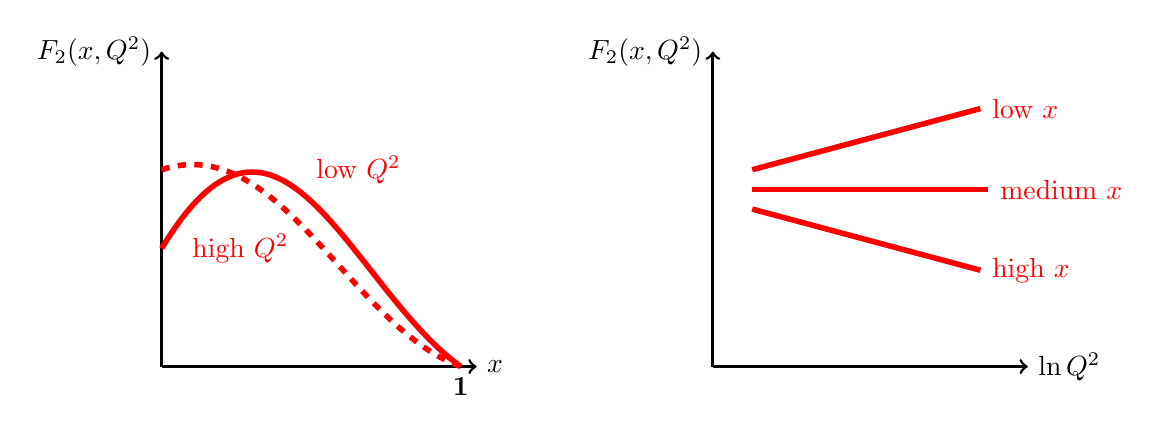
\begin{tikzpicture}[scale=1.0]
\begin{scope}[shift={(0,0)}]
\draw[line width=1pt,black,->] (0,0)  -- +(4,0) node[right] {$x$};
\draw[line width=1pt,black,->] (0,0)  -- +(0,4) node[left] {$F_2(x,Q^2)$};
\node at (3.8,-0.25) {\textbf{1}};
\draw[line width=2pt,red,smooth] (0,1.5)  .. controls (1.5,4) and (2.4,1) .. (3.8,0);
\draw[line width=2pt,red,smooth,dashed] (0,2.5)  .. controls (1.5,3) and (2.4,0.5) .. (3.8,0);
\node[red] at (2.5,2.5) {low $Q^2$};
\node[red] at (1.,1.5) {high $Q^2$};
\end{scope}
%%%%%%%%%%%%%%%%%%%%%%%%%
\begin{scope}[shift={(7,0)}]
\draw[line width=1pt,black,->] (0,0)  -- +(4,0) node[right] {$\ln Q^2$};
\draw[line width=1pt,black,->] (0,0)  -- +(0,4) node[left] {$F_2(x,Q^2)$};
\draw[line width=2pt,red] (0.5,2.5) -- +(15:3) node[right] {low $x$};
\draw[line width=2pt,red] (0.5,2.25) -- +(0:3) node[right] {medium $x$};
\draw[line width=2pt,red] (0.5,2.) -- +(-15:3) node[right] {high $x$};
\end{scope}
\end{tikzpicture}
\caption{Sketch of the expected scaling violation in $F_2$ as a function of
$x$ and $Q^2$.}
\end{figure}
%%%%%%%%%%%%%%%  END FIGURE  %%%%%%%%%%%%%%%%%%%%%%%%%%%%%%
%

\end{document}
